\normalsize
\section{Time Integration}
%\section{Time Integration with Projection Method}

%The solution to Poisson equation is required for the numerical simulation of %incompressible flows using the projection method.
%Three-dimensional incompressible flow with constant density and viscosity is governed %by the Navier-Stokes and continuity equation:
\begin{figure}[htbp]
\hspace{0.0in}
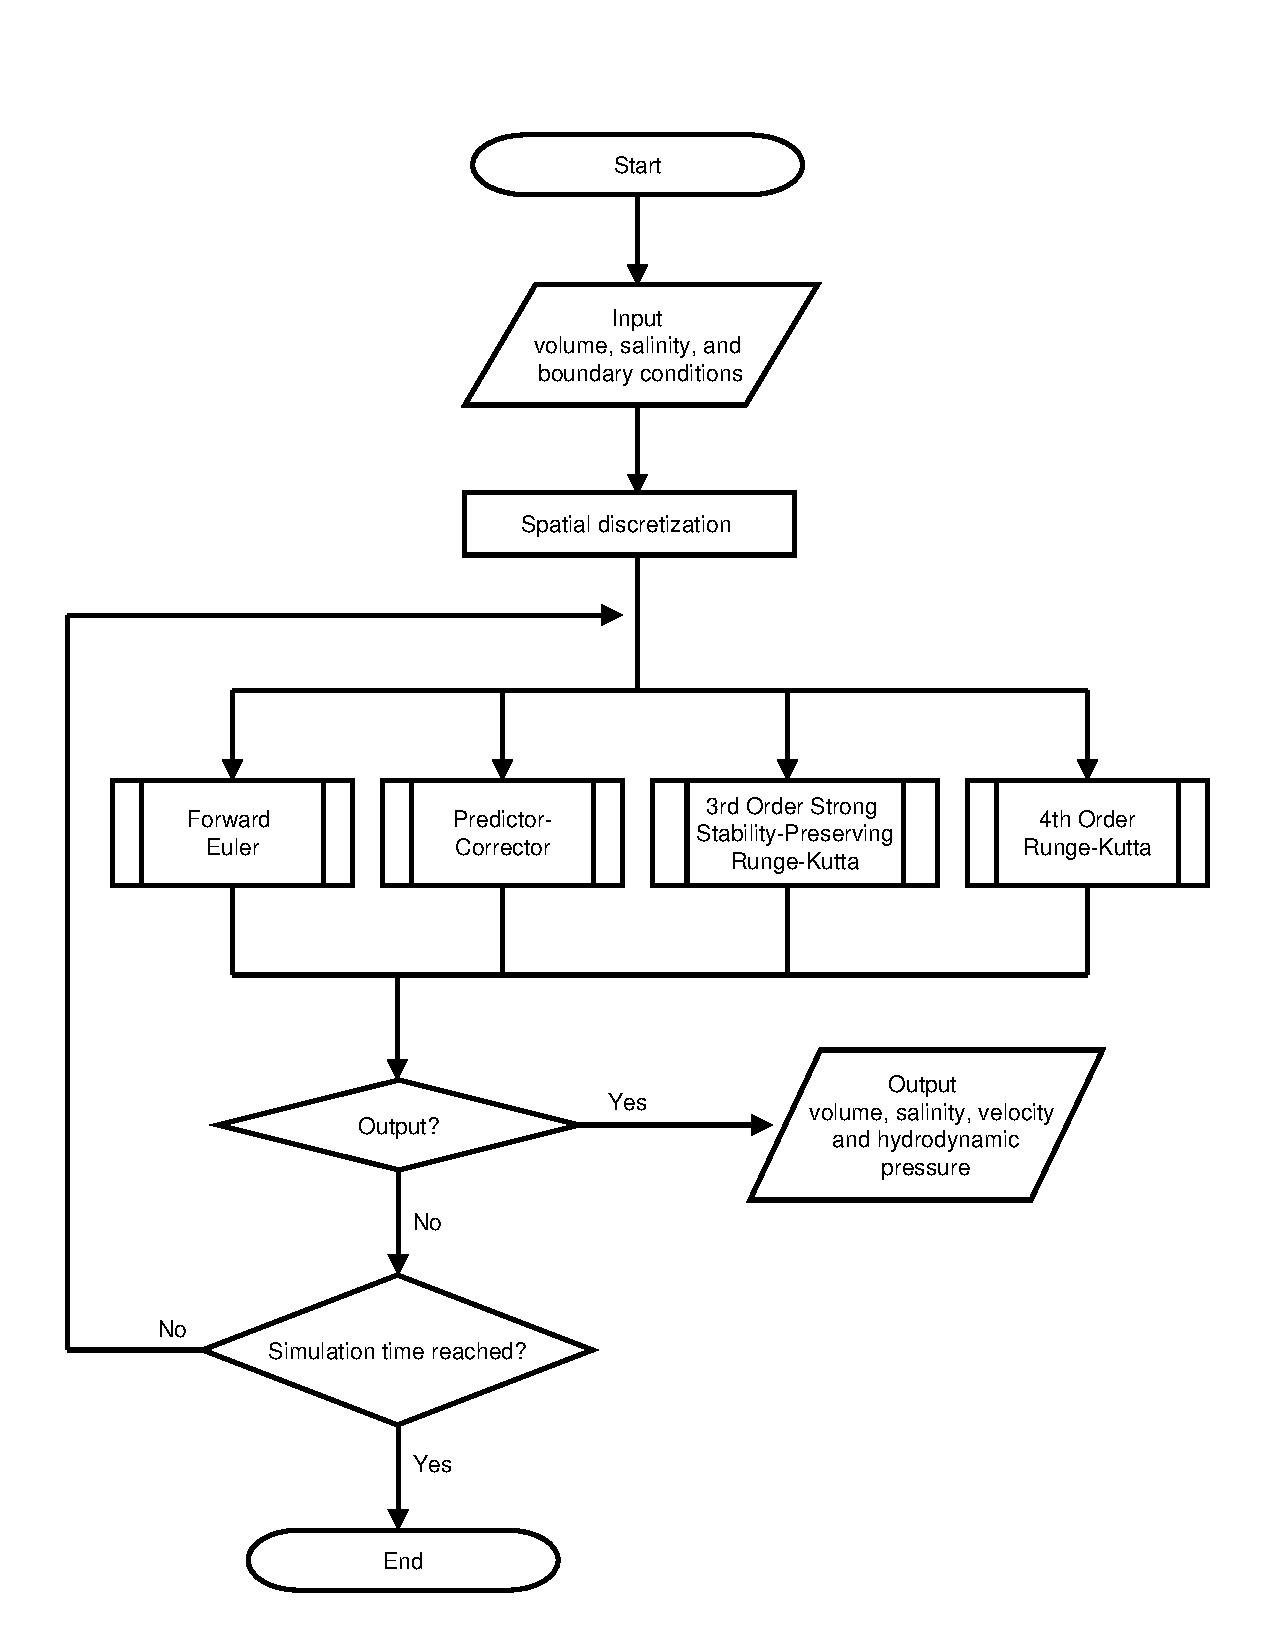
\includegraphics[width=5.8in]{../figures/flowcharts/Main.pdf}
\label{fig:flowchart-main}
\caption{Main flowchart}
\end{figure}

\begin{figure}[htbp]
\hspace{0.25in}
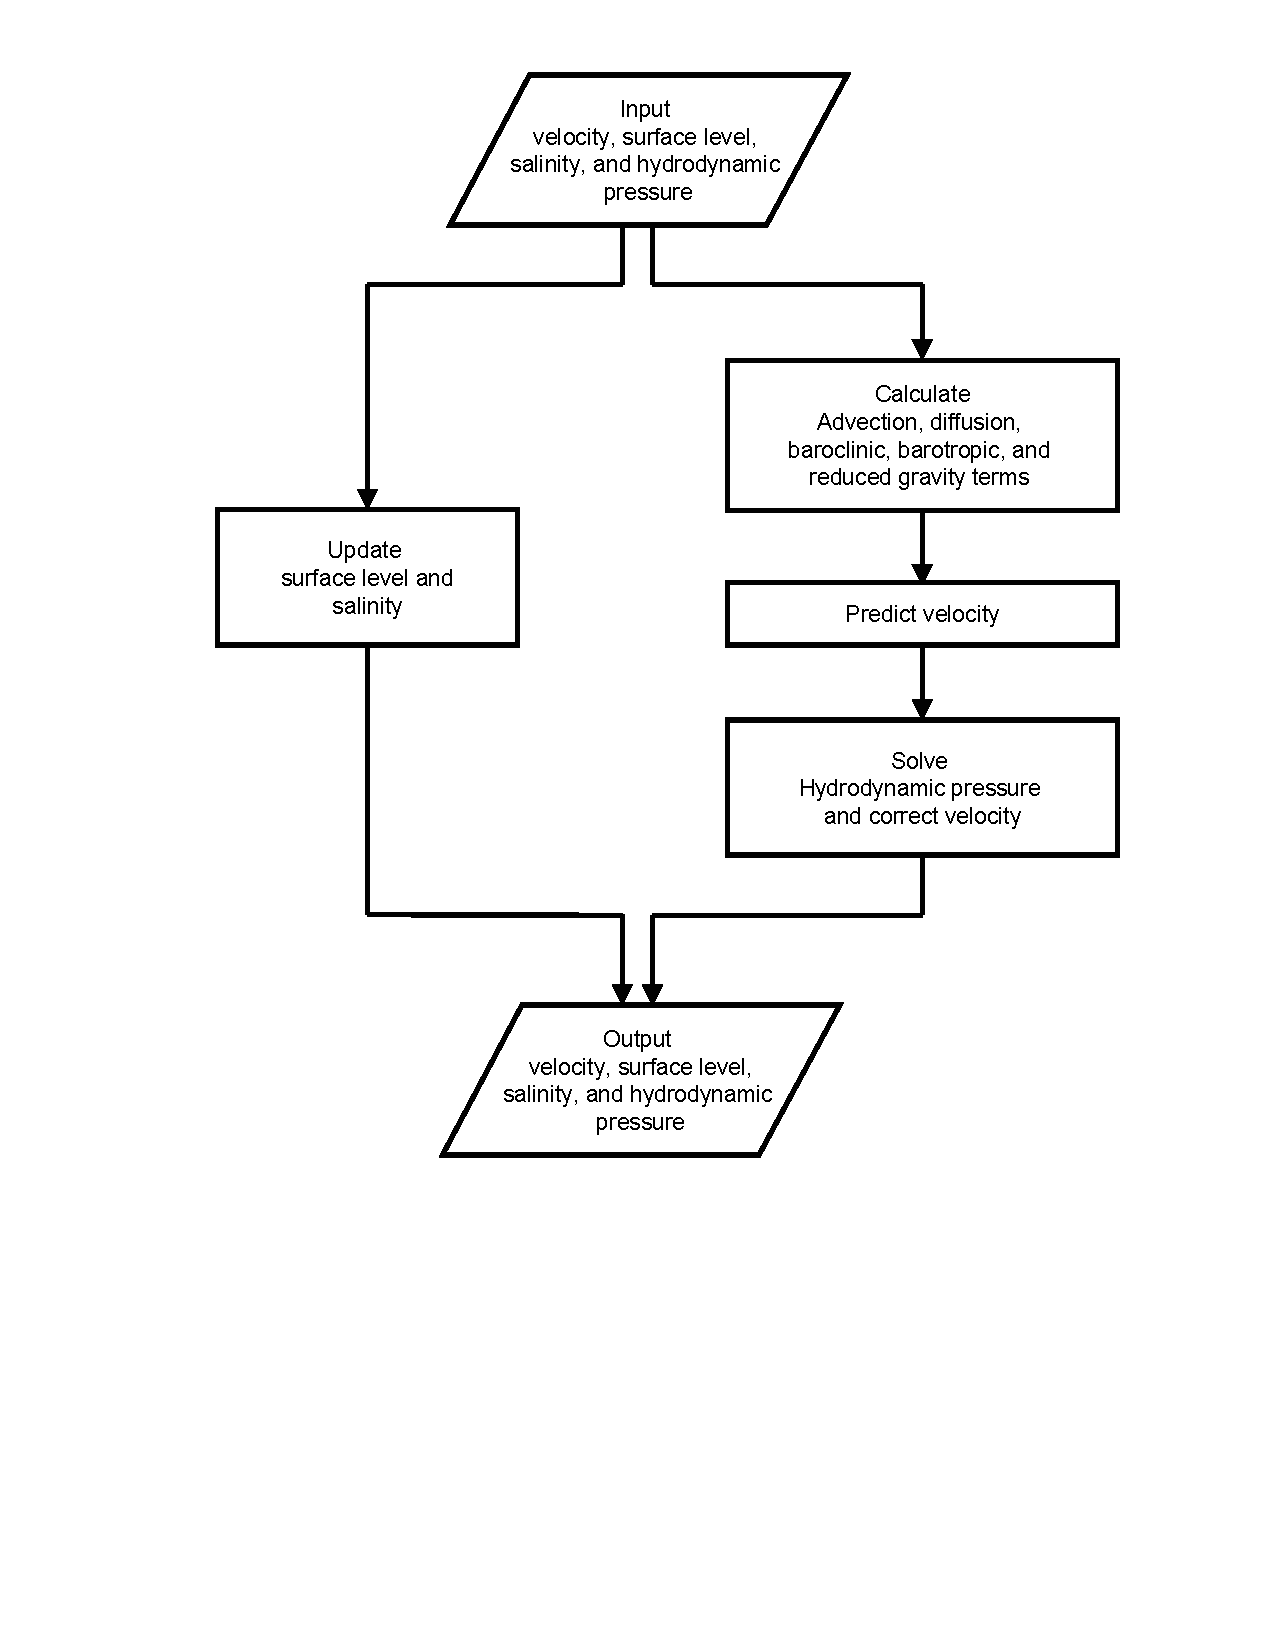
\includegraphics[width=5.0in]{../figures/flowcharts/TimeIntegration-ForwardEuler-text.pdf}
\label{fig:flowchart-ForwardEuler-text}
\caption{Flowchart - time integration. }
\end{figure}

The time integration for incompressible flow is different from the method for compressible flow, because the pressure cannot be calculated directly from the equation of state. Rather, for primitive variables formulation it can be solved from the pressure-Poisson equation resulted from the incompressibility constraint. Chorin proposed the projection method \cite{Chorin1980} that first predicts the velocity field with advection and diffusion but without considering the pressure term, and then the pressure is computed to offset the non-zero divergence of the velocities, forcing them to satisfy the incompressible assumption.

\normalsize
\subsection{Forward-Euler Method}

\begin{figure}[htbp]
\hspace{0.2in}
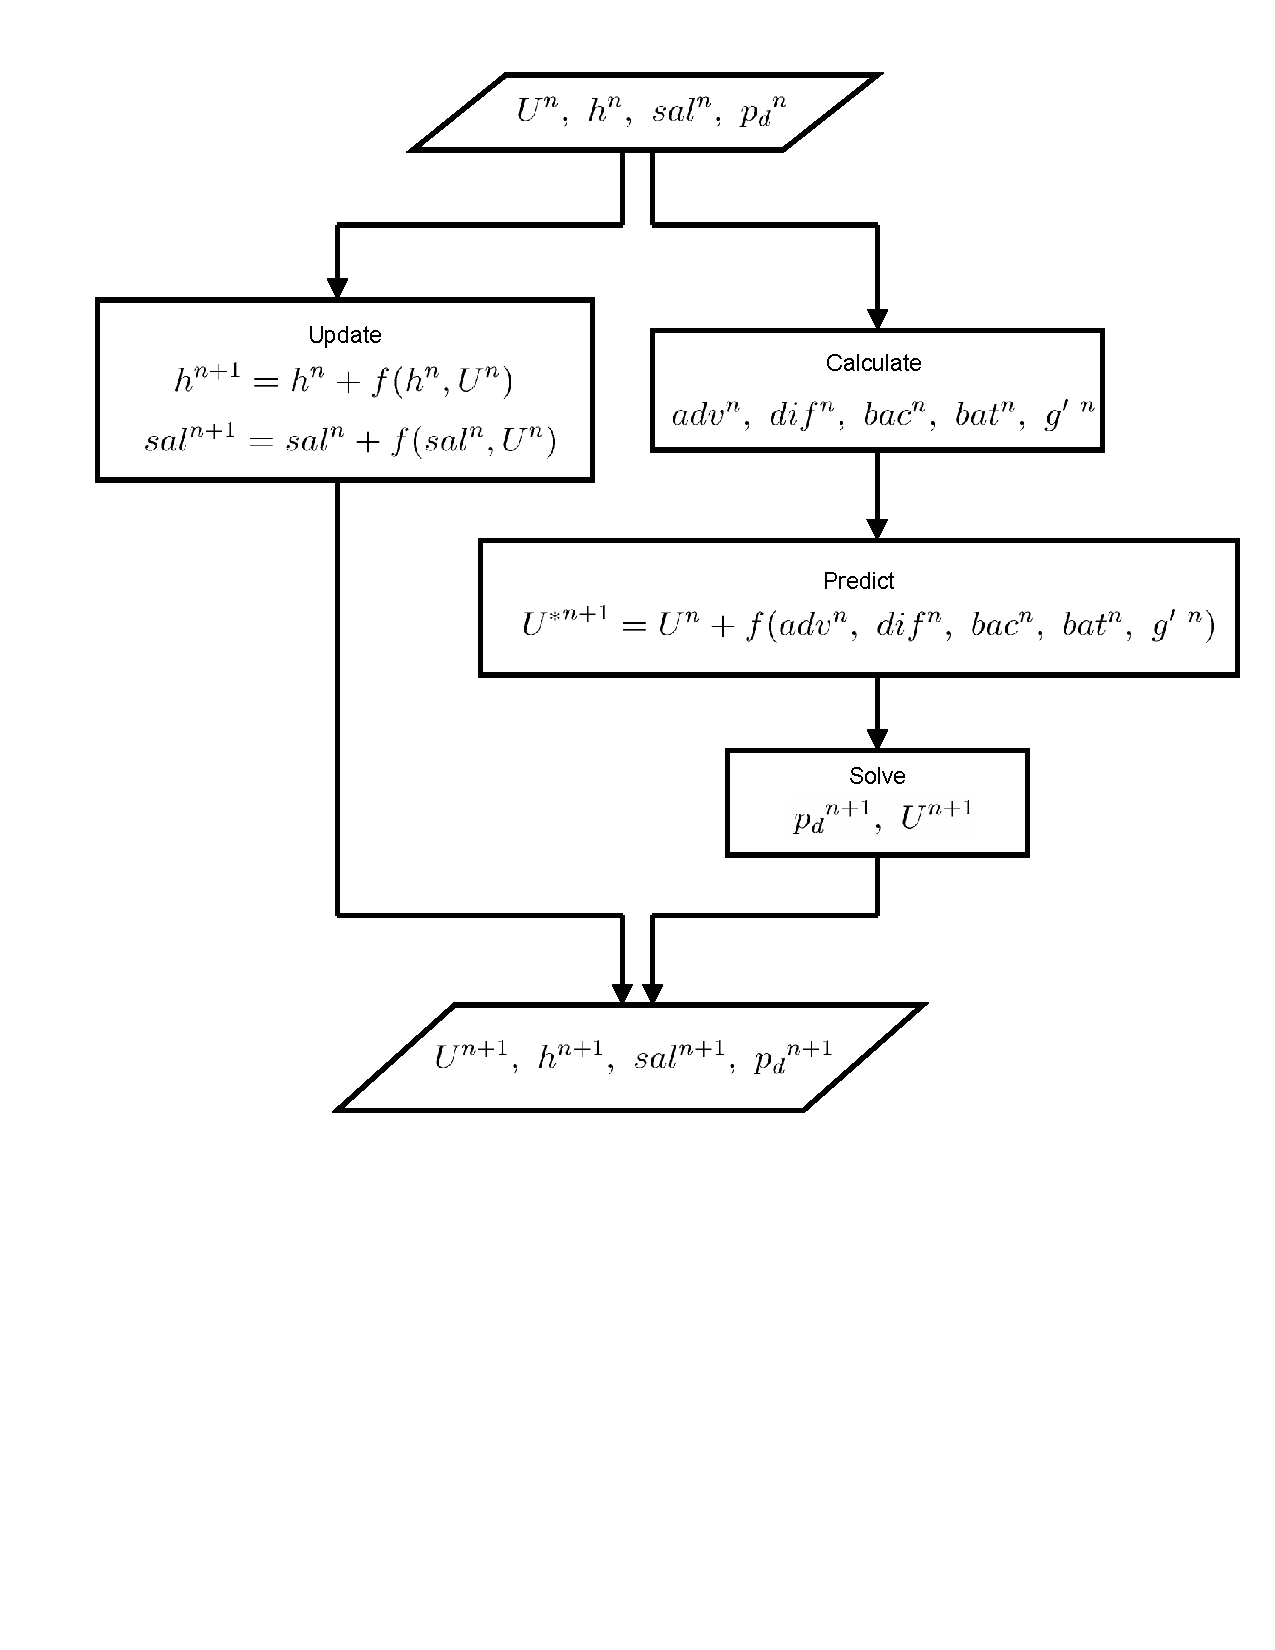
\includegraphics[width=5.5in]{../figures/flowcharts/TimeIntegration-ForwardEuler.pdf}
\label{fig:flowchart-ForwardEuler}
\caption{Flowchart - forward Eular time integration. }
\end{figure}

The Forward-Euler method for time integration is employed to
approximate the Navier-Stokes equations. The estimated velocity, $u^{*}$,
is computed using the advection, diffusion, baroclinic and barotropic terms at the previous time step $n$.
\begin {equation}
u^{*} = u^{n}+ \Delta t  \left\{
-A(u^n)+E(u^n)-\alpha B(u^n)-g\frac{\partial h^n}{\partial
x}%-\frac{1}{\rho_o}\frac{\partial (P^{'s-1})^n}{\partial x}
\right\}
\end{equation}
\begin {equation}
v^{*} = v^{n}+ \Delta t  \left\{
-A(v^n)+E(v^n)-\alpha B(v^n)-g\frac{\partial h^n}{\partial
y}%-\frac{1}{\rho_o}\frac{\partial (P^{'s-1})^n}{\partial x}
\right\}
\end{equation}
\begin {equation}
w^{*} = w^{n}+ \Delta t \cdot \left\{ -A(w^n)+E(w^n) - (1-\alpha)g' \right\}
\end{equation}
where $A$ is the advection term, $E$ is the diffusion term, and $B$ is
the baroclinic term:
\begin{equation}
A(u)=\frac {\partial uu}{\partial x}+ \frac {\partial
uv}{\partial y}+ \frac {\partial uw}{\partial z}
\end{equation}
\begin{equation}
E(u)=\mu (\frac {\partial^2 u}{\partial x^2}+\frac
{\partial^2 u}{\partial y^2}+\frac {\partial^2 u}{\partial z^2})
\end{equation}
\begin{equation}
B(u)=\frac{g}{\rho_o}\int_z^h \frac{\partial \rho}{\partial x} d
\xi
\end{equation}
The time step is limited by Courant-Friedrichs-Lewy condition for the stability criteria of the forward Euler computation,
\be
u \Delta t/\Delta x \leq 1, \ v \Delta t/\Delta y \leq 1, \ w \Delta t/\Delta z \leq 1
\ee
The non-hydrostatic pressure-Poisson equation,
\begin{equation}
\nabla^2 p_d^{n+1} = \frac {\nabla \cdot
\+{u}^*}{\Delta t},
\label{eqn:pressure-poisson-const-den}
\end{equation}
is solved to enforce the incompressibility constraint for the next time step
$n+1$,
\be
\n \cdot \+{u}^{n+1}
\ee
%\begin{equation}
%\frac{\partial u^{n+1}}{\partial x} + \frac{\partial
%v^{n+1}}{\partial y}+\frac{\partial w^{n+1}}{\partial z}= 0
%\end{equation}
Then the velocities at next time step is corrected as:
\be
\+{u}^{n+1}=\+{u}^*-\f{\Delta t}{\rho} \n p_d^{n+1}
\ee
\begin{comment}
\begin{equation}
u^{n+1}=u^*-\frac{\Delta t}{\rho} \frac{\partial
P_d^{n+1}}{\partial x} ,\hspace{0.15in} v^{n+1}=v^*-\frac{\Delta
t}{\rho} \frac{\partial P_d^{n+1}}{\partial y},\hspace{0.15in}
w^{n+1}=w^*-\frac{\Delta t}{\rho} \frac{\partial
P^{n+1}_d}{\partial z}
\end{equation}
\end{comment}

However, the residuals of the pressure correction may not
disappear at steady state. This weakness can be avoided by
including the pressure term to predict the intermediate velocities,
\begin {equation}
u^{*} = u^{n}+ \Delta t  \left\{
-A(u^n)+E(u^n)-\alpha B(u^n)-g\frac{\partial h^n}{\partial
x}-\frac{1}{\rho}\frac{\partial p_d^n}{\partial x} \right\}
\label{eqn:chap-FlowModel-momentum-u}
\end{equation}
\begin {equation}
v^{*} = v^{n}+ \Delta t  \left\{
-A(v^n)+E(v^n)-\alpha B(v^n)-g\frac{\partial h^n}{\partial
y}-\frac{1}{\rho}\frac{\partial p_d^n}{\partial y} \right\}
\label{eqn:chap-FlowModel-momentum-v}
\end{equation}
\begin {equation}
w^{*} = w^{n}+ \Delta t \cdot \left\{
-A(w^n)+E(w^n)-(1-\alpha)g'-\frac{1}{\rho}\frac{\partial p_d^n}{\partial z}
\right\}
\label{eqn:chap-FlowModel-momentum-w}
\end{equation}
Therefore the pressure-Poisson equation becomes:
\begin{equation}
\nabla^2 (p_d^{n+1}-p_d^{n}) = \frac{\nabla \cdot
\+{u}^*}{\Delta t}
\end{equation}
And the corrected velocity is:
\begin{equation}
\+{u}^{n+1}=\+{u}^*- \frac{\Delta t}{\rho}
\nabla (p_d^{n+1}-p_d^n)
\end{equation}

\normalsize
\subsection{Runge-Kutta Methods}
The general form of Runge-Kutta method \cite{Chapra2006} can be written as:
\be
y^{n+1}=y^n +(a_1 k_1+a_2 k_2+\cdots+a_{m+1} k_{m+1}) \Delta t
\ee
where the next time step $y^{n+1}$ is evaluated by a series of predictions:
\ba
k_1&=&f(t^n, \ y^n) \\
k_2&=&f(t^n+p_1 \Delta t, \ y^n+ q_{11}k_1 \Delta t) \\
k_3&=&f[t^n+p_2 \Delta t, \ y^n+(q_{21}k_1+q_{22}k_2)\Delta t] \\
& & \cdots \nn \\
& & \cdots \nn \\
k_{m+1}&=&f[t^n+p_{m} \Delta t, \ y^n+(q_{m1}k_1+q_{m2}k_2+\cdots +q_{mm}k_m)\Delta t]
\ea
Those coefficients $a's$, $p's$, and $q's$ are chosen to satisfy the required order of accuracy in the Taylor series expansion.

\normalsize
\subsubsection*{Midpoint Method}

\begin{figure}[htbp]
\hspace{0in}
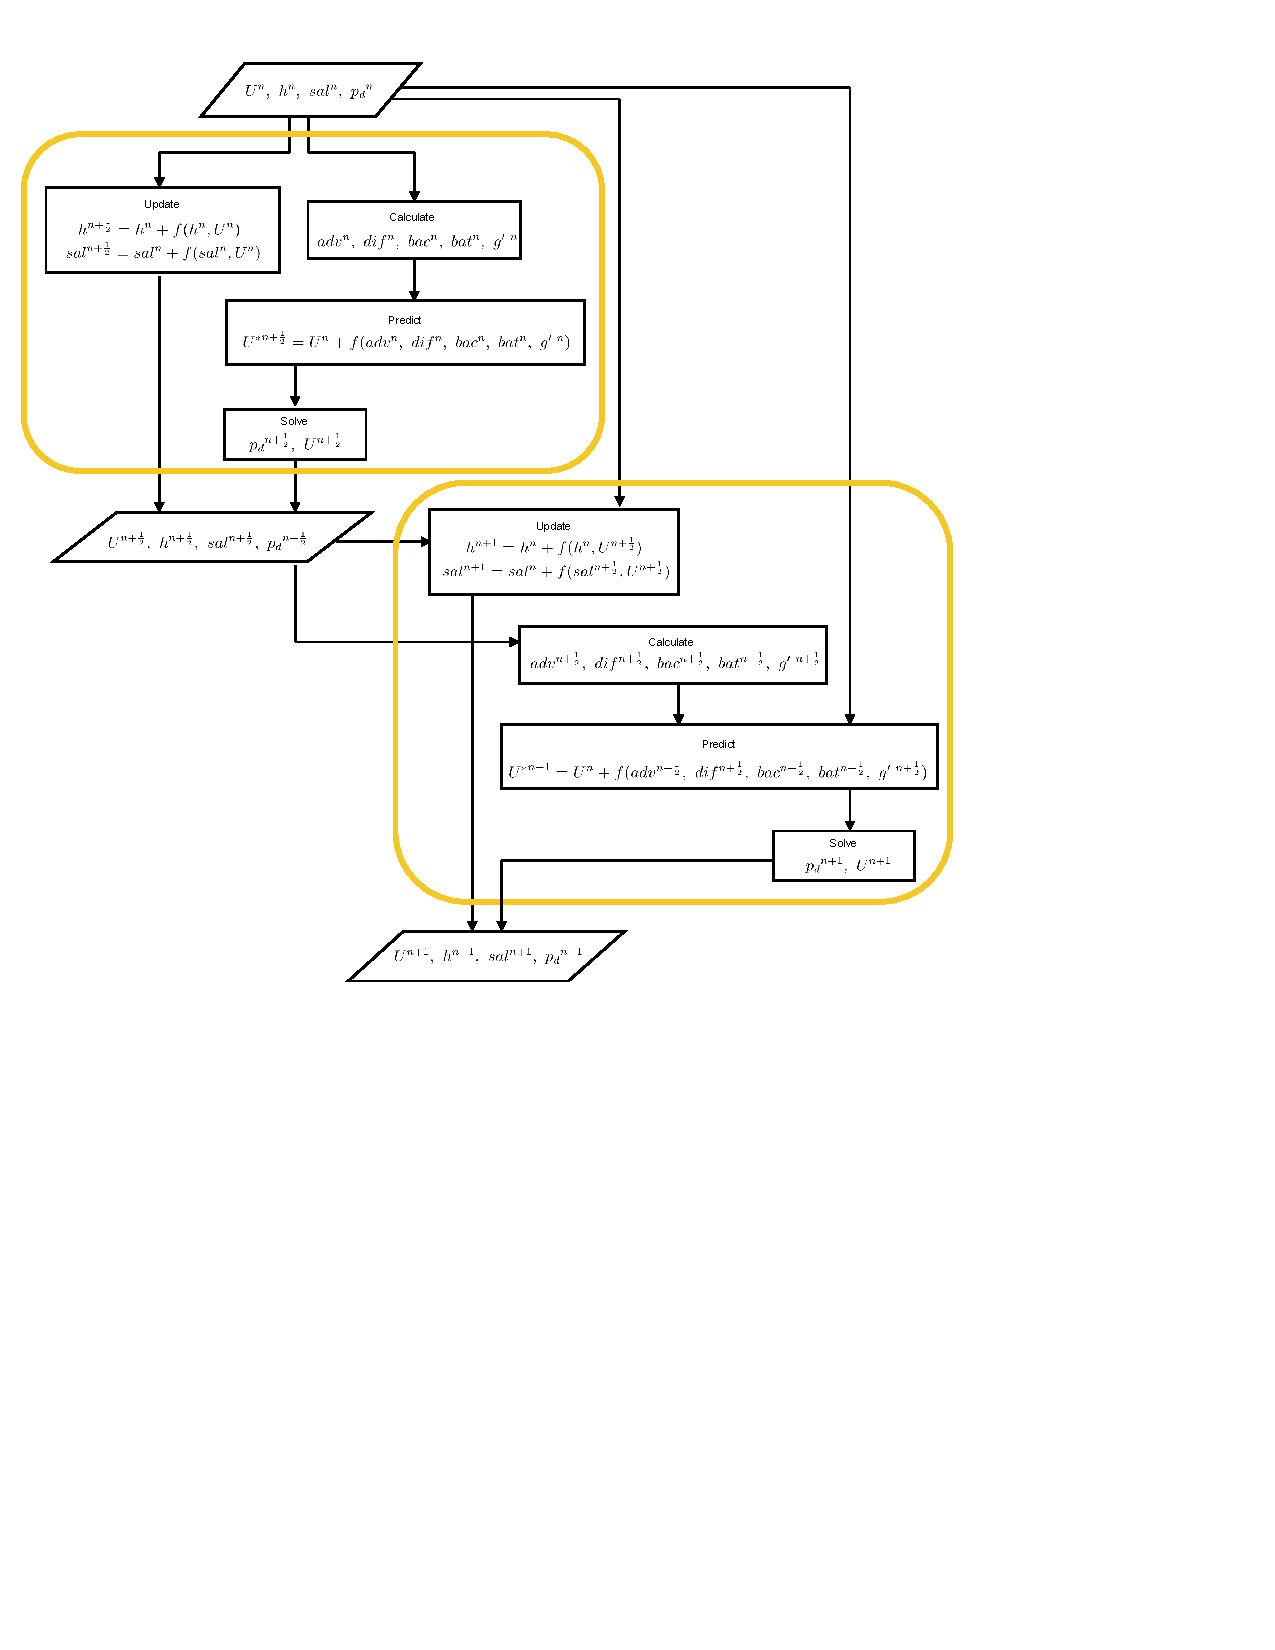
\includegraphics[width=5.95in]{../figures/flowcharts/TimeIntegration-2nd.pdf}
\label{fig:flowchart-MidPoint}
\caption{Flowchart - midpoint time integration. }
\end{figure}

Midpoint method is a second order Runge-Kutta method with the coefficient $a_1=0$, $a_2=1$, $p_1=\f{1}{2}$, and $q_{11}=\f{1}{2}$:
\ba
y^{n+1}&=&y^n + k_2 \Delta t \\
k_1 &=& f(t^n, \ y^n) \\
k_2 &=& f(t^n+\f{1}{2} \Delta t, \ y^n+\f{1}{2}k_1 \Delta t )
\ea
The above equations are implemented in the flow model for multi-variable functions:
\ba
\mathbf{Y}^{n+\f{1}{2}}&=&\mathbf{Y}^n+F( \ \mathbf{Y}^n, \ \f{\Delta t}{2} \ )  \\
\mathbf{Y}^{n+1}&=&\mathbf{Y}^n + F( \ \mathbf{Y}^{n+\f{1}{2}}, \ \Delta t \ )
\ea
where $F$ is the time integration subroutine including the hydrodynamic pressure solver; the vector $Y$ contains the variables of velocities, water level $h$, salinity $Sal$, and hydrodynamic pressure $p_d$. These variables are the basic elements in the advection, diffusion, barotropic, and baroclinic functions.
\be
\mathbf{Y} = ( \ u,\ v,\ w,\ h,\ Sal,\ p_d \ )
\ee

\normalsize
\subsubsection*{Classical Fourth-Order Runge-Kutta Method}

\begin{figure}[htbp]
\hspace{0in}
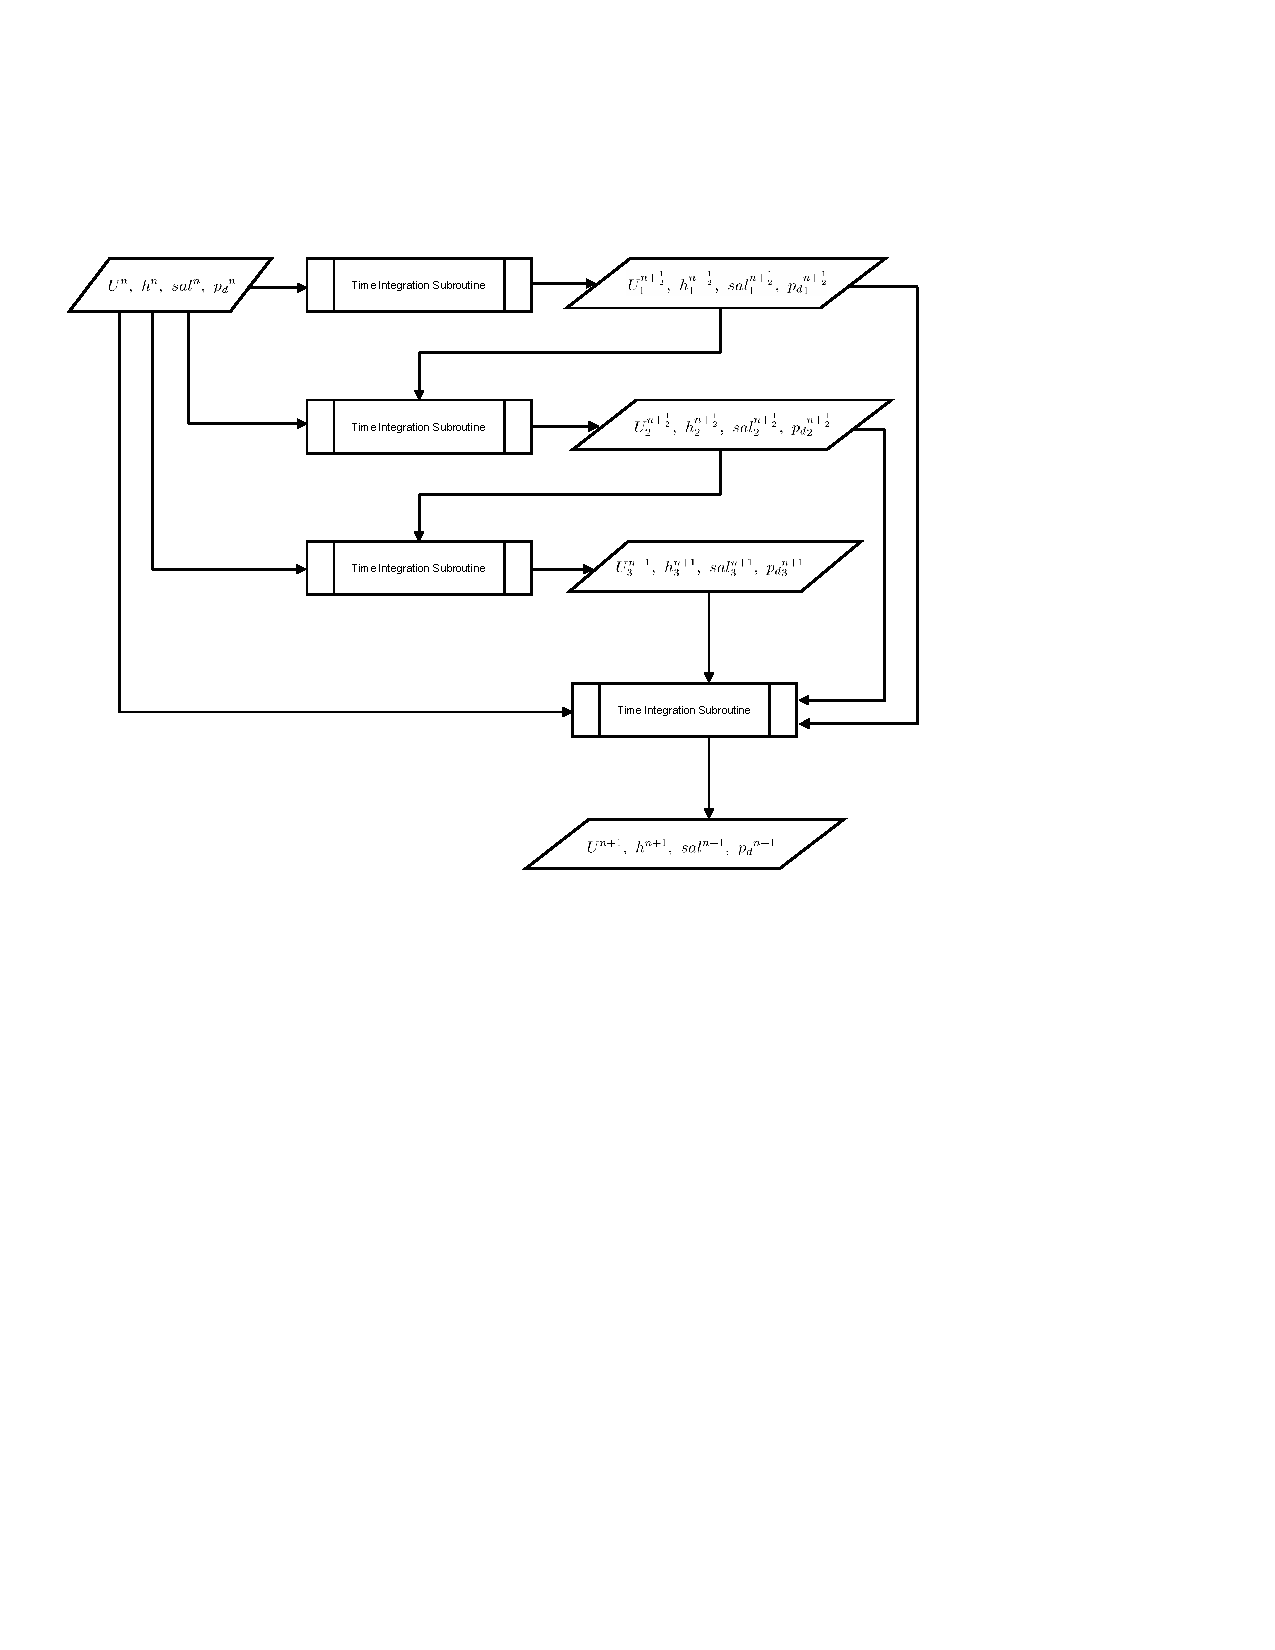
\includegraphics[width=5.8in]{../figures/flowcharts/TimeIntegration-RK4.pdf}
\label{fig:flowchart-RK4}
\caption{Flowchart - RK4 time integration }
\end{figure}

The classical version of the fourth-order Runge-Kutta method is:
\ba
y^{n+1}&=&y^n + \f{1}{6}(k_1+2k_2+2k_3+k_4) \Delta t \\
k_1 &=& f(t^n, \ y^n) \\
k_2 &=& f(t^n+\f{1}{2} \Delta t, \ y^n+\f{1}{2}k_1 \Delta t ) \\
k_3 &=& f(t^n+\f{1}{2} \Delta t, \ y^n+\f{1}{2}k_2 \Delta t ) \\
k_4 &=& f(t^n+\Delta t, \ y^n+ k_3 \Delta t )
\ea

Implement the above equations for the vector $\mathbf{Y} = ( \ u,\ v,\ w,\ h,\ Sal,\ p_d \ )$:
\ba
\mathbf{Y}_1&=&\mathbf{Y}^n+F( \ \mathbf{Y}^n, \ \f{\Delta t}{2} \ )  \\
\mathbf{Y}_2&=&\mathbf{Y}^n+F( \ \mathbf{Y}_1, \ \f{\Delta t}{2} \ )  \\
\mathbf{Y}_3&=&\mathbf{Y}^n+F( \ \mathbf{Y}_2, \ \Delta t \ )  \\
\mathbf{Y}^{n+1}&=&\mathbf{Y}^n+F( \ \f{\mathbf{Y}^n+2\mathbf{Y}_1+2\mathbf{Y}_2+\mathbf{Y}_3}{6}, \ \Delta t \ )
\ea

\normalsize
\subsection{Strong-Stability Preserving Runge-Kutta Method}

\begin{figure}[htbp]
\hspace{0in}
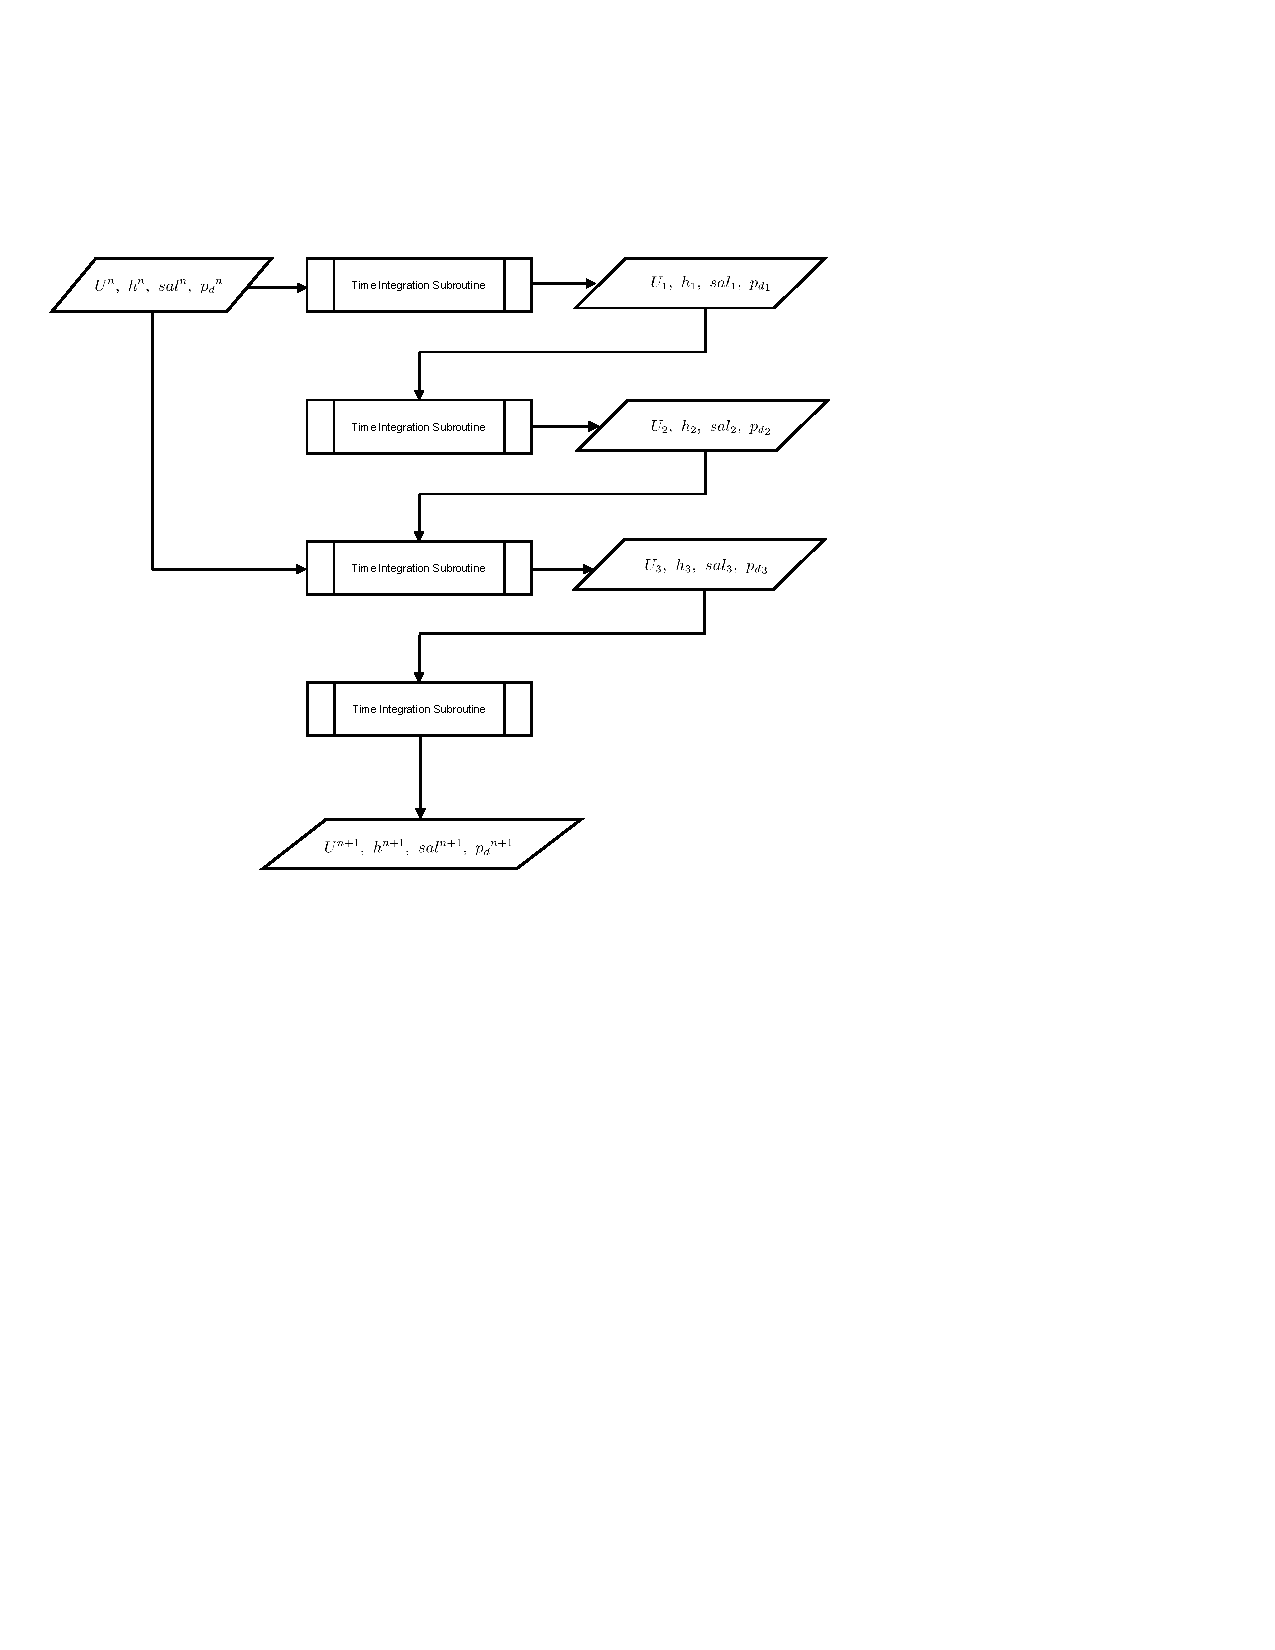
\includegraphics[width=5.8in]{../figures/flowcharts/TimeIntegration-SSPRK.pdf}
\label{fig:flowchart-RK4}
\caption{Flowchart - strong stability preserving RK 3rd order 4-step time integration }
\end{figure}

Strong-stability preserving means that some given norm of the solution sequence to that numerical method is non-increasing. A four-stage, order-three explicit strong- stability-preserving Runge-Kutta method with non-negative coefficients \cite{Ruuth2004} \cite{Macdonald2003} is
\ba
y_1 &=& y^n+\f{\Delta t}{2} f(y^n) \nonumber \\
y_2 &=& y_1+\f{\Delta t}{2} f(y_1) \nn \\
y_3 &=& \f{2}{3}y^n + \f{1}{3}y_2 + \f{\Delta t}{6} f(y_2) \nn \\
y^{n+1} &=& y_3+\f{\Delta t}{2} f(y_3)
\ea

\ba
\mathbf{Y}_1 &=& \mathbf{Y}^n+ F( \ \mathbf{Y}^n, \ \f{\Delta t}{2} \ ) \nonumber \\
\mathbf{Y}_2 &=& \mathbf{Y}_1+ F( \ \mathbf{Y}_1, \ \f{\Delta t}{2} \ ) \nn \\
\mathbf{Y}_3 &=& \f{2}{3}\mathbf{Y}^n + \f{1}{3}\mathbf{Y}_2 + F( \ \mathbf{Y}_2, \ \f{\Delta t}{6} \ ) \nn \\
\mathbf{Y}^{n+1} &=& \mathbf{Y}_3+ F( \ \mathbf{Y}_3, \ \f{\Delta t}{2} \ )
\ea

It can be seen that the CFL coefficient \cite{Courant1967} for this method is 2 \cite{Ruuth2002}. 